% !TEX spellcheck = en_US



% ~~~~~~~~~~~~~~~~~~~~~~~~~~~~~~~~~~~~~~~ V
% (NC) 2026 Haluk Bingol
% github.com/halukbingol/LaTeX-Templates
%
% Licensees may copy, distribute, display, and perform the work and make derivative works 
% and remixes based on it only for non-commercial purposes. 
% ~~~~~~~~~~~~~~~~~~~~~~~~~~~~~~~~~~~~~~~ A




% =====================================================================
%  Java on the Command Line -- The Concepts
%  ---------------------------------------------------------------------
%  Built on hbCisLaTeXTemplate.tex with the libraries in ../../hblib/.
%  Programs and their outputs are read from codeoutput/:
%     codeoutput/<Name>.java   the program
%     codeoutput/<Name>.in     keyboard input (optional)
%     codeoutput/<Name>.txt    what it printed, made by:  sh run_examples.sh
% =====================================================================

\documentclass[aspectratio=169,10pt,compress]{beamer}

% ~~~~~~~~~~~~~~~~~~~~~~~~~~~~~~~~~~~~~~~~~~~~~~~~~~~~~~~~~~~~~~~~~ V hblib
	\usepackage{../../hblib/hblibPresentation} % lib presentation: theme, i/N, \hSection, algorithm2e, ...
	\usepackage{../../hblib/hblibCodeoutput} % lib code + output: \lstcode, \lstcodedown, ...
	\usepackage{../../hblib/hblibDatastructures} % lib data structures: \hString, \hStack, \hQueue
% ~~~~~~~~~~~~~~~~~~~~~~~~~~~~~~~~~~~~~~~~~~~~~~~~~~~~~~~~~~~~~~~~~ A hblib


% xcolor, array (and the L{width} column), listings, tikz and algorithm2e come from the hblib libraries
\usepackage[T1]{fontenc}
\usepackage{lmodern}
\usepackage{booktabs}

\definecolor{gitred}{RGB}{240,80,50}
\newcommand{\cmd}[1]{\texttt{\color{gitred}#1}}

\usetikzlibrary{fit, shapes.geometric}
\tikzset{
  box/.style={draw, thick, rounded corners, align=center, font=\small, inner sep=5pt},
  file/.style={draw, thick, fill=blue!8, align=center, font=\ttfamily\small, minimum height=0.8cm, inner sep=4pt},
  tool/.style={-{Stealth[length=2.5mm]}, thick},
  lbl/.style={font=\scriptsize\sffamily, text=gray!70!black}
}

% ---------------------------------------------------------------------
\title{Java on the Command Line}
\subtitle{The Concepts}
\author[Bingol]{Haluk O. Bingol}

\institute[FCIS]{
    Faculty of Computer and Information Sciences\\
    Yeditepe University
}
\date{
	{\tiny \hbTimeStamp}
}

\begin{document}




% ~~~~~~~~~~~~~~~~~~~~~~~~~~~~~~~~~~~~~~ V frm
\begin{frame}[t,fragile]
  \titlepage
\end{frame}
% ~~~~~~~~~~~~~~~~~~~~~~~~~~~~~~~~~~~~~~ A frm




% ~~~~~~~~~~~~~~~~~~~~~~~~~~~~~~~~~~~~~~ V frm
\begin{frame}[t,fragile] \frametitle{Outline}
  \tableofcontents[hideallsubsections]
\end{frame}
% ~~~~~~~~~~~~~~~~~~~~~~~~~~~~~~~~~~~~~~ A frm

% ~~~~~~~~~~~~~~~~~~~~~~~~~~~~~~~~~~~~~~ V
\hSection[CLI]{What Is a Command Line?}{}{}
% ~~~~~~~~~~~~~~~~~~~~~~~~~~~~~~~~~~~~~~ A

% ~~~~~~~~~~~~~~~~~~~~~~~~~~~~~~~~~~~~~~ V
\subsection[Shell]{Terminal and shell}
% ~~~~~~~~~~~~~~~~~~~~~~~~~~~~~~~~~~~~~~ A




% ~~~~~~~~~~~~~~~~~~~~~~~~~~~~~~~~~~~~~~ V frm
\begin{frame}[t,fragile] \frametitle{Terminal, shell, command}
  \begin{columns}[T]
    \begin{column}{0.5\textwidth}
      \begin{itemize}\small
        \item A \textbf{terminal} is the window; a \textbf{shell} is the program in it that reads your commands
        \item The \textbf{prompt} waits for a command line:
              \texttt{program argument argument ...}
        \item The shell finds the program, starts it, and passes the \textbf{arguments}
        \item Every shell has a \textbf{working directory}: relative file names start there
      \end{itemize}


% +++++++++++++++++++++++++++++++++++++++ V lst
%: -Lst.
\begin{lstlisting}[style=codesnippet, language={}]
javac -d out Hello.java
^^^^^ ^^^^^^^^^^^^^^^^^^^^
program   three arguments
\end{lstlisting}
% +++++++++++++++++++++++++++++++++++++++ A lst



    \end{column}
    \begin{column}{0.46\textwidth}
      \footnotesize
      \begin{tabular}{@{}L{0.17\textwidth}L{0.4\textwidth}L{0.32\textwidth}@{}}
        \toprule
                  & \textbf{Windows} & \textbf{macOS} \\
        \midrule
        terminal  & Windows Terminal & Terminal \\
        shell     & Command Prompt (\texttt{cmd}), PowerShell & \texttt{zsh} (default), \texttt{bash} \\
        prompt    & \texttt{C:\textbackslash Users\textbackslash ayse>} & \texttt{ayse@mac \textasciitilde \%} \\
        list files & \texttt{dir} & \texttt{ls} \\
        path sep. & \texttt{\textbackslash}  & \texttt{/} \\
        \bottomrule
      \end{tabular}

      \vspace{0.5em}
      \small In these slides a \texttt{\$} line is a command; lines below it are its output.
    \end{column}
  \end{columns}
\end{frame}
% ~~~~~~~~~~~~~~~~~~~~~~~~~~~~~~~~~~~~~~ A frm

% ~~~~~~~~~~~~~~~~~~~~~~~~~~~~~~~~~~~~~~ V
\subsection[Why]{Why the command line?}
% ~~~~~~~~~~~~~~~~~~~~~~~~~~~~~~~~~~~~~~ A




% ~~~~~~~~~~~~~~~~~~~~~~~~~~~~~~~~~~~~~~ V frm
\begin{frame}[t,fragile] \frametitle{Why learn Java on the command line?}
  \begin{columns}[T]
    \begin{column}{0.48\textwidth}
      \begin{block}{Understanding}
        \small An IDE's ``Run'' button does exactly these steps: compile with \texttt{javac}, run with \texttt{java}.
        When the IDE fails, you can still see what is going on.
      \end{block}
      \begin{block}{Automation}
        \small Commands can be put in scripts: build, test and run with one command, every time the same way.
      \end{block}
    \end{column}
    \begin{column}{0.48\textwidth}
      \begin{block}{Servers and the cloud}
        \small Servers and containers have no screen. Java applications are started there with \texttt{java -jar app.jar}.
      \end{block}
      \begin{block}{Build tools}
        \small Maven, Gradle and continuous integration (GitHub Actions, \dots) call the same JDK tools.
      \end{block}
    \end{column}
  \end{columns}
\end{frame}
% ~~~~~~~~~~~~~~~~~~~~~~~~~~~~~~~~~~~~~~ A frm

% ~~~~~~~~~~~~~~~~~~~~~~~~~~~~~~~~~~~~~~ V
\hSection[JDK]{Where javac, java and jar Come From}{}{}
% ~~~~~~~~~~~~~~~~~~~~~~~~~~~~~~~~~~~~~~ A

% ~~~~~~~~~~~~~~~~~~~~~~~~~~~~~~~~~~~~~~ V
\subsection[Layers]{JDK, JRE, JVM}
% ~~~~~~~~~~~~~~~~~~~~~~~~~~~~~~~~~~~~~~ A




% ~~~~~~~~~~~~~~~~~~~~~~~~~~~~~~~~~~~~~~ V frm
\begin{frame}[t,fragile] \frametitle{JDK, JRE and JVM}
  \begin{columns}[T]
    \begin{column}{0.5\textwidth}
      \begin{center}
      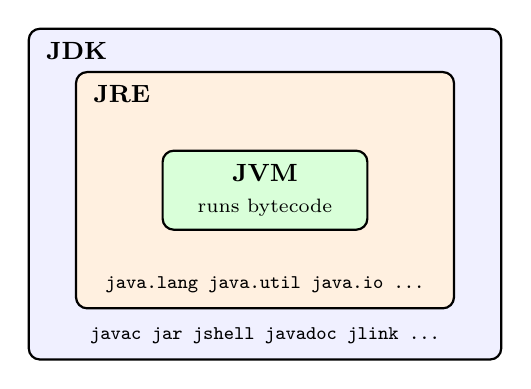
\begin{tikzpicture}
        \draw[thick, rounded corners, fill=blue!6] (-3,-2.1) rectangle (3,2.1);
        \node[anchor=north west, font=\small\bfseries] at (-2.9,2.05) {JDK};
        \node[font=\ttfamily\scriptsize] at (0,-1.8) {javac jar jshell javadoc jlink ...};
        \draw[thick, rounded corners, fill=orange!12] (-2.4,-1.45) rectangle (2.4,1.55);
        \node[anchor=north west, font=\small\bfseries] at (-2.3,1.5) {JRE};
        \node[font=\ttfamily\scriptsize] at (0,-1.15) {java.lang java.util java.io ...};
        \node[box, fill=green!15, minimum width=2.6cm, minimum height=1.0cm] at (0,0.05) {\textbf{JVM}\\ \scriptsize runs bytecode};
      \end{tikzpicture}
      \end{center}
    \end{column}
    \begin{column}{0.46\textwidth}
      \begin{itemize}\small
        \item \textbf{JVM} (Java Virtual Machine): loads and executes \texttt{.class} files
        \item \textbf{JRE} (runtime): JVM + the standard library (\texttt{java.lang}, \texttt{java.util}, \dots)
        \item \textbf{JDK} (development kit): JRE + development tools: \texttt{javac}, \texttt{jar}, \texttt{jshell}, \dots
        \item To \textbf{write} programs you need a JDK; since Java 11 most vendors ship only the JDK
        \item \texttt{java} is in both; \texttt{javac} only in the JDK
      \end{itemize}
    \end{column}
  \end{columns}
\end{frame}
% ~~~~~~~~~~~~~~~~~~~~~~~~~~~~~~~~~~~~~~ A frm

% ~~~~~~~~~~~~~~~~~~~~~~~~~~~~~~~~~~~~~~ V
\subsection[Pipeline]{From source to a running program}
% ~~~~~~~~~~~~~~~~~~~~~~~~~~~~~~~~~~~~~~ A




% ~~~~~~~~~~~~~~~~~~~~~~~~~~~~~~~~~~~~~~ V frm
\begin{frame}[t,fragile] \frametitle{From source code to a running program}
  \begin{center}
  \begin{tikzpicture}[x=1cm, y=1cm]
    \node[file] (src) at (0,0) {Hello.java\\ \scriptsize\sffamily source (text)};
    \node[file, fill=orange!12] (cls) at (5,0) {Hello.class\\ \scriptsize\sffamily bytecode};
    \node[file, fill=yellow!20] (jar) at (5,-2) {app.jar\\ \scriptsize\sffamily zip of classes};
    \node[box, fill=green!12, minimum width=3.2cm] (jvm) at (10.2,0) {\textbf{JVM}\\ \scriptsize load, verify, interpret, JIT};
    \draw[tool] (src) -- node[above, font=\ttfamily\small]{javac} node[below, lbl]{compile} (cls);
    \draw[tool] (cls) -- node[above, font=\ttfamily\small]{java} node[below, lbl]{run} (jvm);
    \draw[tool] (cls) -- node[right, font=\ttfamily\small]{jar} node[left, lbl]{package} (jar);
    \draw[tool] (jar) -| node[below, pos=0.25, font=\ttfamily\small]{java -jar} (jvm);
    \node[lbl, align=center] at (10.2,-1.3) {same \texttt{.class}/\texttt{.jar} on\\ Windows, macOS, Linux};
  \end{tikzpicture}
  \end{center}
  \begin{itemize}\small
    \item \texttt{javac} checks types and translates once; errors here are \textbf{compile-time} errors
    \item \texttt{java} starts a JVM, loads the main class and calls \texttt{main}; errors here are \textbf{run-time} errors (exceptions)
    \item Bytecode is portable: compile on macOS, run on Windows (``write once, run anywhere'')
  \end{itemize}
\end{frame}
% ~~~~~~~~~~~~~~~~~~~~~~~~~~~~~~~~~~~~~~ A frm

% ~~~~~~~~~~~~~~~~~~~~~~~~~~~~~~~~~~~~~~ V
\subsection[Tools]{The tools in the JDK}
% ~~~~~~~~~~~~~~~~~~~~~~~~~~~~~~~~~~~~~~ A




% ~~~~~~~~~~~~~~~~~~~~~~~~~~~~~~~~~~~~~~ V frm
\begin{frame}[t,fragile] \frametitle{The tools in \texttt{JDK/bin}}
  \small
  \begin{tabular}{@{}L{0.14\textwidth}L{0.48\textwidth}L{0.3\textwidth}@{}}
    \toprule
    \textbf{Tool} & \textbf{Does} & \textbf{Example} \\
    \midrule
    \texttt{javac}    & compiles \texttt{.java} to \texttt{.class}            & \texttt{javac -d out Hello.java} \\
    \texttt{java}     & starts the JVM and runs a class or jar                  & \texttt{java -cp out Hello} \\
    \texttt{jar}      & creates and reads \texttt{.jar} archives              & \texttt{jar --list --file app.jar} \\
    \texttt{jshell}   & interactive Java (REPL)                               & \texttt{jshell} \\
    \texttt{javadoc}  & HTML documentation from comments                      & \texttt{javadoc -d docs ...} \\
    \texttt{javap}    & shows what is inside a \texttt{.class}                & \texttt{javap -c Hello} \\
    \texttt{jdeps}    & lists dependencies of classes/jars                    & \texttt{jdeps app.jar} \\
    \texttt{jlink}    & builds a small custom runtime                         & \texttt{jlink --add-modules ...} \\
    \texttt{jpackage} & builds an installer or app bundle                     & \texttt{jpackage --input ...} \\
    \texttt{jcmd}, \texttt{jfr} & inspect a running JVM                       & \texttt{jcmd <pid> Thread.print} \\
    \bottomrule
  \end{tabular}
\end{frame}
% ~~~~~~~~~~~~~~~~~~~~~~~~~~~~~~~~~~~~~~ A frm

% ~~~~~~~~~~~~~~~~~~~~~~~~~~~~~~~~~~~~~~ V
\subsection[Get]{Getting a JDK}
% ~~~~~~~~~~~~~~~~~~~~~~~~~~~~~~~~~~~~~~ A




% ~~~~~~~~~~~~~~~~~~~~~~~~~~~~~~~~~~~~~~ V frm
\begin{frame}[t,fragile] \frametitle{Getting a JDK}
  \begin{columns}[T]
    \begin{column}{0.48\textwidth}
      \small Java is open source (\textbf{OpenJDK}). Several vendors build and ship it:
      \begin{itemize}\small
        \item Eclipse \textbf{Temurin} (\texttt{adoptium.net}): free, widely used in teaching
        \item Oracle JDK, Amazon Corretto, Microsoft Build of OpenJDK, Azul Zulu, \dots
      \end{itemize}
      \textbf{Versions}: a new one every 6 months; \textbf{LTS} (long-term support) releases are 8, 11, 17, 21, 25.
      Courses usually use the latest LTS.
    \end{column}
    \begin{column}{0.48\textwidth}
      \begin{block}{Windows}
        \footnotesize \texttt{.msi} installer (tick \emph{Set JAVA\_HOME}, \emph{Add to PATH}), or
        \cmd{winget install EclipseAdoptium.Temurin.21.JDK}.
        Installs to \texttt{C:\textbackslash Program Files\textbackslash Eclipse Adoptium\textbackslash jdk-21...}
      \end{block}
      \begin{block}{macOS}
        \footnotesize \texttt{.pkg} installer (Apple silicon: \emph{aarch64}), or \cmd{brew install --cask temurin@21}.
        Installs to \texttt{/Library/Java/JavaVirtualMachines/}
      \end{block}
    \end{column}
  \end{columns}
\end{frame}
% ~~~~~~~~~~~~~~~~~~~~~~~~~~~~~~~~~~~~~~ A frm




% ~~~~~~~~~~~~~~~~~~~~~~~~~~~~~~~~~~~~~~ V frm
\begin{frame}[t,fragile] \frametitle{Which Java do I have?}
  \lstoutput[basicstyle=\ttfamily\tiny]{codeoutput/Versions.txt}

  \vspace{0.2em}
  \small These slides were made with OpenJDK 21 (an Ubuntu build); on your computer the vendor line differs.
  \texttt{java} and \texttt{javac} should report the \textbf{same} version.
\end{frame}
% ~~~~~~~~~~~~~~~~~~~~~~~~~~~~~~~~~~~~~~ A frm

% ~~~~~~~~~~~~~~~~~~~~~~~~~~~~~~~~~~~~~~ V
\hSection[PATH]{How the Shell Finds java}{}{}
% ~~~~~~~~~~~~~~~~~~~~~~~~~~~~~~~~~~~~~~ A

% ~~~~~~~~~~~~~~~~~~~~~~~~~~~~~~~~~~~~~~ V
\subsection[PATH]{PATH and JAVA\_HOME}
% ~~~~~~~~~~~~~~~~~~~~~~~~~~~~~~~~~~~~~~ A




% ~~~~~~~~~~~~~~~~~~~~~~~~~~~~~~~~~~~~~~ V frm
\begin{frame}[t,fragile] \frametitle{PATH and JAVA\_HOME}
  \begin{columns}[T]
    \begin{column}{0.5\textwidth}
      \small Typing \texttt{javac} makes the shell search the folders in the \textbf{PATH} environment variable,
      in order, for a program with that name. The first match wins.
      \begin{center}
      \begin{tikzpicture}[x=1cm, y=0.62cm]
        \node[box, fill=gray!10, font=\ttfamily\small] (cmd) at (0,0) {javac};
        \node[draw, fill=gray!8, font=\ttfamily\scriptsize, minimum width=3.2cm, anchor=west] at (1.6,0) {/usr/local/bin};
        \node[draw, fill=gray!8, font=\ttfamily\scriptsize, minimum width=3.2cm, anchor=west] at (1.6,-1) {/usr/bin};
        \node[draw, fill=green!15, font=\ttfamily\scriptsize, minimum width=3.2cm, anchor=west] at (1.6,-2) {\$JAVA\_HOME/bin};
        \draw[tool] (cmd.east) -- (1.6,0);
        \draw[tool, gray] (1.4,0) |- (1.6,-1);
        \draw[tool, green!50!black] (1.2,0) |- (1.6,-2);
        \node[lbl, anchor=west] at (4.9,-2) {found};
      \end{tikzpicture}
      \end{center}
      \textbf{JAVA\_HOME} is the JDK's folder; tools such as Maven and Gradle use it.
    \end{column}
    \begin{column}{0.46\textwidth}
      \begin{block}{Windows}
        \footnotesize Settings $\to$ \emph{Edit the system environment variables} $\to$ \emph{Environment Variables}.
        Check: \cmd{where java}, \cmd{echo \%JAVA\_HOME\%}. Open a \textbf{new} window after changes.
      \end{block}
      \begin{block}{macOS}
        \footnotesize In \texttt{\textasciitilde/.zshrc}:\\
        \texttt{export JAVA\_HOME=\$(/usr/libexec/java\_home -v 21)}\\
        \texttt{export PATH="\$JAVA\_HOME/bin:\$PATH"}\\
        Check: \cmd{which java}, \cmd{/usr/libexec/java\_home -V} (all JDKs).
      \end{block}
    \end{column}
  \end{columns}
\end{frame}
% ~~~~~~~~~~~~~~~~~~~~~~~~~~~~~~~~~~~~~~ A frm

% ~~~~~~~~~~~~~~~~~~~~~~~~~~~~~~~~~~~~~~ V
\hSection[Classpath]{Classes, Packages and the Classpath}{}{}
% ~~~~~~~~~~~~~~~~~~~~~~~~~~~~~~~~~~~~~~ A

% ~~~~~~~~~~~~~~~~~~~~~~~~~~~~~~~~~~~~~~ V
\subsection[Packages]{Packages are folders}
% ~~~~~~~~~~~~~~~~~~~~~~~~~~~~~~~~~~~~~~ A




% ~~~~~~~~~~~~~~~~~~~~~~~~~~~~~~~~~~~~~~ V frm
\begin{frame}[t,fragile] \frametitle{Packages are folders}
  \begin{columns}[T]
    \begin{column}{0.48\textwidth}


% +++++++++++++++++++++++++++++++++++++++ V lst
%: -Lst.
\begin{lstlisting}[style=codesnippet, language=Java]
package edu.yeditepe.cse;

public class Main { ... }
\end{lstlisting}
% +++++++++++++++++++++++++++++++++++++++ A lst



      \small The \textbf{fully qualified name} is \texttt{edu.yeditepe.cse.Main}. Its class file must be at
      \texttt{edu/yeditepe/cse/Main.class} \textbf{relative to a classpath entry}.
    \end{column}
    \begin{column}{0.48\textwidth}


% +++++++++++++++++++++++++++++++++++++++ V lst
%: -Lst.
\begin{lstlisting}[style=codesnippet, language={}]
out/          <- on the classpath
`-- edu/
    `-- yeditepe/
        `-- cse/
            |-- Main.class
            `-- Util.class
\end{lstlisting}
% +++++++++++++++++++++++++++++++++++++++ A lst



      \small Run with the \textbf{class name}, not a file name:\\
      \texttt{java -cp out edu.yeditepe.cse.Main}
    \end{column}
  \end{columns}
\end{frame}
% ~~~~~~~~~~~~~~~~~~~~~~~~~~~~~~~~~~~~~~ A frm

% ~~~~~~~~~~~~~~~~~~~~~~~~~~~~~~~~~~~~~~ V
\subsection[Classpath]{The classpath}
% ~~~~~~~~~~~~~~~~~~~~~~~~~~~~~~~~~~~~~~ A




% ~~~~~~~~~~~~~~~~~~~~~~~~~~~~~~~~~~~~~~ V frm
\begin{frame}[t,fragile] \frametitle{The classpath}
  \begin{columns}[T]
    \begin{column}{0.52\textwidth}
      \small The JVM looks for classes in a list of places, the \textbf{classpath}:
      \begin{itemize}\small
        \item folders (\texttt{out}) and jar files (\texttt{lib/json.jar})
        \item given with \texttt{-cp} (or \texttt{--class-path}); default: the current folder \texttt{.}
        \item separator: \texttt{;} on Windows, \texttt{:} on macOS/Linux
        \item searched in order; the first class found wins
      \end{itemize}
      \begin{alertblock}{The most common error}
        \small \texttt{Error: Could not find or load main class ...} means: not on the classpath, or a wrong name.
      \end{alertblock}
    \end{column}
    \begin{column}{0.44\textwidth}
      \begin{block}{Windows}
        \footnotesize \texttt{java -cp out;lib\textbackslash json.jar app.Main}
      \end{block}
      \begin{block}{macOS}
        \footnotesize \texttt{java -cp out:lib/json.jar app.Main}
      \end{block}
      \small Java's own classes (\texttt{String}, \texttt{ArrayList}) come from the runtime and need no classpath entry.
    \end{column}
  \end{columns}
\end{frame}
% ~~~~~~~~~~~~~~~~~~~~~~~~~~~~~~~~~~~~~~ A frm

% ~~~~~~~~~~~~~~~~~~~~~~~~~~~~~~~~~~~~~~ V
\subsection[Jar]{JAR files}
% ~~~~~~~~~~~~~~~~~~~~~~~~~~~~~~~~~~~~~~ A




% ~~~~~~~~~~~~~~~~~~~~~~~~~~~~~~~~~~~~~~ V frm
\begin{frame}[t,fragile] \frametitle{JAR files}
  \begin{columns}[T]
    \begin{column}{0.48\textwidth}
      \small A \textbf{JAR} (Java ARchive) is a \textbf{zip file} of \texttt{.class} files and resources, plus a manifest:


% +++++++++++++++++++++++++++++++++++++++ V lst
%: -Lst.
\begin{lstlisting}[style=codesnippet, language={}]
app.jar
|-- META-INF/MANIFEST.MF
|-- edu/yeditepe/cse/Main.class
|-- edu/yeditepe/cse/Util.class
`-- messages.properties
\end{lstlisting}
% +++++++++++++++++++++++++++++++++++++++ A lst



    \end{column}
    \begin{column}{0.48\textwidth}
      \small \texttt{META-INF/MANIFEST.MF} is a small text file:


% +++++++++++++++++++++++++++++++++++++++ V lst
%: -Lst.
\begin{lstlisting}[style=codesnippet, language={}]
Manifest-Version: 1.0
Main-Class: edu.yeditepe.cse.Main
Class-Path: lib/json.jar
\end{lstlisting}
% +++++++++++++++++++++++++++++++++++++++ A lst



      \begin{itemize}\small
        \item With \texttt{Main-Class}, the jar is \textbf{executable}: \texttt{java -jar app.jar}
        \item One file to copy, mail or deploy
        \item Libraries are distributed as jars
      \end{itemize}
    \end{column}
  \end{columns}
\end{frame}
% ~~~~~~~~~~~~~~~~~~~~~~~~~~~~~~~~~~~~~~ A frm

% ~~~~~~~~~~~~~~~~~~~~~~~~~~~~~~~~~~~~~~ V
\hSection[Interface]{A Program and Its Surroundings}{}{}
% ~~~~~~~~~~~~~~~~~~~~~~~~~~~~~~~~~~~~~~ A

% ~~~~~~~~~~~~~~~~~~~~~~~~~~~~~~~~~~~~~~ V
\subsection[Streams]{Arguments, streams, exit code}
% ~~~~~~~~~~~~~~~~~~~~~~~~~~~~~~~~~~~~~~ A




% ~~~~~~~~~~~~~~~~~~~~~~~~~~~~~~~~~~~~~~ V frm
\begin{frame}[t,fragile] \frametitle{What a command-line program receives and returns}
  \begin{center}
  \begin{tikzpicture}[x=1cm, y=1cm]
    \node[box, fill=green!12, minimum width=3.4cm, minimum height=2.2cm] (p) at (0,0) {\textbf{your program}\\[2pt] \ttfamily\scriptsize main(String[] args)};
    \node[box, fill=blue!6, anchor=east] (a) at (-3.4,1.1) {arguments\\ \ttfamily\scriptsize args[0], args[1]};
    \node[box, fill=blue!6, anchor=east] (i) at (-3.4,-0.2) {standard input\\ \ttfamily\scriptsize System.in};
    \node[box, fill=blue!6, anchor=east] (e) at (-3.4,-1.4) {environment\\ \ttfamily\scriptsize System.getenv, -D};
    \node[box, fill=orange!10, anchor=west] (o) at (3.4,1.0) {standard output\\ \ttfamily\scriptsize System.out};
    \node[box, fill=red!10, anchor=west] (r) at (3.4,-0.2) {standard error\\ \ttfamily\scriptsize System.err};
    \node[box, fill=yellow!15, anchor=west] (x) at (3.4,-1.4) {exit code\\ \ttfamily\scriptsize System.exit(n)};
    \foreach \s in {a,i,e} \draw[tool] (\s.east) -- (p.west |- \s.east);
    \foreach \t in {o,r,x} \draw[tool] (p.east |- \t.west) -- (\t.west);
  \end{tikzpicture}
  \end{center}
  \small
  \begin{itemize}
    \item The shell can \textbf{redirect}: \texttt{java App < in.txt > out.txt 2> err.txt} (same on Windows and macOS)
    \item Exit code \texttt{0} means success; anything else is a failure. Check it with
          \texttt{echo \$?} (macOS) or \texttt{echo \%ERRORLEVEL\%} (Windows Command Prompt)
  \end{itemize}
\end{frame}
% ~~~~~~~~~~~~~~~~~~~~~~~~~~~~~~~~~~~~~~ A frm

% ~~~~~~~~~~~~~~~~~~~~~~~~~~~~~~~~~~~~~~ V
\subsection[Launch]{What java does}
% ~~~~~~~~~~~~~~~~~~~~~~~~~~~~~~~~~~~~~~ A




% ~~~~~~~~~~~~~~~~~~~~~~~~~~~~~~~~~~~~~~ V frm
\begin{frame}[t,fragile] \frametitle{What happens when you type \texttt{java -cp out app.Main}}
  \begin{enumerate}\small
    \item The shell finds \texttt{java} on the PATH and passes it the arguments \texttt{-cp}, \texttt{out}, \texttt{app.Main}
    \item The \textbf{launcher} reads options (\texttt{-cp}, \texttt{-D}, \texttt{-Xmx}, \dots) and starts a JVM
    \item The JVM loads \texttt{app.Main} through the class loaders (from \texttt{out/app/Main.class})
    \item The bytecode is \textbf{verified}, then \texttt{public static void main(String[] args)} is called with the remaining arguments
    \item Classes are loaded \textbf{lazily}, when first used; hot code is compiled to machine code by the \textbf{JIT}
    \item When \texttt{main} returns (and no other non-daemon thread runs) or \texttt{System.exit(n)} is called, the JVM exits;
          an uncaught exception gives exit code 1
  \end{enumerate}
  \vspace{0.3em}
  \begin{block}{Shortcut since Java 11}
    \small \texttt{java Hello.java} compiles a single source file in memory and runs it: no \texttt{.class} file is written.
  \end{block}
\end{frame}
% ~~~~~~~~~~~~~~~~~~~~~~~~~~~~~~~~~~~~~~ A frm

% ~~~~~~~~~~~~~~~~~~~~~~~~~~~~~~~~~~~~~~ V
\hSection[Summary]{Summary}{}{}
% ~~~~~~~~~~~~~~~~~~~~~~~~~~~~~~~~~~~~~~ A

% ~~~~~~~~~~~~~~~~~~~~~~~~~~~~~~~~~~~~~~ V
\subsection[Ideas]{Big ideas}
% ~~~~~~~~~~~~~~~~~~~~~~~~~~~~~~~~~~~~~~ A




% ~~~~~~~~~~~~~~~~~~~~~~~~~~~~~~~~~~~~~~ V frm
\begin{frame}[t,fragile] \frametitle{Big ideas}
  \small
  \begin{tabular}{@{}L{0.2\textwidth}L{0.72\textwidth}@{}}
    \toprule
    \textbf{Idea} & \textbf{In one sentence} \\
    \midrule
    JDK          & Gives you \texttt{javac}, \texttt{java}, \texttt{jar} and more; get it from a vendor such as Temurin. \\
    PATH         & The shell finds tools through PATH; \texttt{JAVA\_HOME} points to the JDK. \\
    \texttt{javac} & Source $\to$ bytecode; reports compile-time errors. \\
    \texttt{java}  & Starts a JVM and runs \texttt{main} of a \textbf{class} (by name) or a jar. \\
    Packages     & Package names are folder paths below a classpath entry. \\
    Classpath    & Where the JVM looks for classes: \texttt{-cp}, separated by \texttt{;} (Windows) or \texttt{:} (macOS). \\
    \texttt{jar}   & A zip of classes with a manifest; \texttt{Main-Class} makes it runnable. \\
    I/O          & Arguments, stdin, stdout, stderr, exit code, environment. \\
    \bottomrule
  \end{tabular}
\end{frame}
% ~~~~~~~~~~~~~~~~~~~~~~~~~~~~~~~~~~~~~~ A frm




% ~~~~~~~~~~~~~~~~~~~~~~~~~~~~~~~~~~~~~~ V frm
\begin{frame}[t,fragile] \frametitle{Check yourself}
  \begin{enumerate}\small
    \item \hQuestion{Which program turns \texttt{Hello.java} into \texttt{Hello.class}?}
          \onslide<2->{\hRemark{\texttt{javac}, the Java compiler.}}
    \item \hQuestion{Why does \texttt{java Hello.class} fail?}
          \onslide<3->{\hRemark{\texttt{java} expects a class \textbf{name}; it looks for a class called \texttt{Hello.class}.}}
    \item \hQuestion{Where must the class \texttt{a.b.C} be, if the classpath is \texttt{out}?}
          \onslide<4->{\hRemark{In \texttt{out/a/b/C.class}.}}
    \item \hQuestion{\texttt{javac} is ``not recognized'' but \texttt{java} works. Why?}
          \onslide<5->{\hRemark{Only a JRE is on the PATH, or the JDK's \texttt{bin} folder is missing from PATH.}}
    \item \hQuestion{What makes \texttt{java -jar app.jar} know which class to start?}
          \onslide<6->{\hRemark{The \texttt{Main-Class} line in \texttt{META-INF/MANIFEST.MF}.}}
    \item \hQuestion{How can a script tell that a Java program failed?}
          \onslide<7->{\hRemark{From its exit code: non-zero means failure.}}
  \end{enumerate}
\end{frame}
% ~~~~~~~~~~~~~~~~~~~~~~~~~~~~~~~~~~~~~~ A frm




% ~~~~~~~~~~~~~~~~~~~~~~~~~~~~~~~~~~~~~~ V frm
\begin{frame}[t,fragile]
	\begin{center}
		\vspace{4cm}
		\hRemark{\Huge Questions?}
	\end{center}
\end{frame}
% ~~~~~~~~~~~~~~~~~~~~~~~~~~~~~~~~~~~~~~ A frm



\end{document}
